\documentclass[11pt,a4paper]{article}
\usepackage[margin=2.2cm]{geometry}
\usepackage{amsmath,amssymb,booktabs,longtable,xcolor,hyperref,graphicx}
\usepackage[T1]{fontenc}
\hypersetup{colorlinks=true,linkcolor=blue,urlcolor=blue}
\newcommand{\code}[1]{\texttt{\small #1}}
\setlength{\parskip}{0.35em}
\graphicspath{{../figures/}}

\title{\vspace{-1.5em}\textbf{The real increment test}\\[0.2em]
       \large the ocean absorbs 99\% of it --- but PISM is collapsing\\[0.3em]
       \normalsize\textit{2026-07-13, evening. Follows \texttt{dynamics\_seam\_2026-07-13}.}}
\author{}
\date{}

\begin{document}
\maketitle
\vspace{-2.5em}

\begin{abstract}
\noindent
The previous note established that the CORE3(observed)$\to$PISM cavity swap is a one-off monster
that production never has to survive, and that cold-starting the ocean on PISM's cavity sidesteps
it. That was done, chunk~1 ran a clean model year, PISM ran its 10~years, and for the first time
the remap was asked to carry \emph{a year of genuine spun-up ocean dynamics across a real PISM
increment}. It failed --- but the way it failed inverts the conclusion. \textbf{The ocean absorbed
$\sim$99\% of the change} (CFLz \emph{peaked and then decayed}; $\eta$ had zero NaN; only
\textbf{17 of 209\,172 nodes} misbehaved). What is actually wrong is upstream: \textbf{PISM is in
massive disequilibrium and is shedding its ice shelves}. The Ross front retreats $\approx$4$^\circ$
of latitude ($\approx$440~km) in a \emph{single} 10-yr leg, and \textbf{1399 nodes have their ice
removed outright}, ringing the whole Antarctic margin. The ``gentle 22\,m increment'' framing used
to justify this whole strategy was wrong.
\end{abstract}

\section{What the increment test actually did}

Chunk-3 (awiesm3 1901) crashed at \textbf{day 15.66} ($\eta_n$ NaN check). But read the diagnostics
before concluding anything --- they look nothing like the monster swap:

\begin{center}
\begin{tabular}{@{}lll@{}}
\toprule
 & \textbf{monster swap} (CORE3$\to$PISM) & \textbf{real increment} (this leg) \\
\midrule
CFLz over time & $4.46 \to 6.43 \to 7.25 \to 9.24$ & $5.26 \to \mathbf{5.78} \to 5.40 \to 4.51 \to \mathbf{4.15}$ \\
               & \textbf{monotonic runaway} & \textbf{peaks, then DECAYS} \\
died at        & day $\sim$4 & day 15.7 \\
$\eta_n$ NaN   & yes & \textbf{none} --- all 209\,172 nodes finite \\
$|\eta|>3$ nodes & 3611, basin-wide, radiating & \textbf{17}, one tight cluster \\
 & mostly \emph{unchanged} nodes & \textbf{all 17 on changed nodes} \\
\bottomrule
\end{tabular}
\end{center}

\noindent
The CFLz \emph{decays}: the ocean is \emph{absorbing} the geometry change, not running away from it.
And the 17 offending nodes share one signature exactly:

\begin{center}
\begin{tabular}{@{}lr@{}}
\toprule
all 17 ringing nodes & \code{ulev 17 $\to$ 1} \\
i.e. & 16 ocean levels opened \emph{at once} \\
$\eta$ values & $+24.4,\ -17.9,\ +15.9,\ +8.3,\ +5.3$ \\
 & alternating sign $\Rightarrow$ grid-scale \textbf{checkerboard} \\
\bottomrule
\end{tabular}
\end{center}

\noindent
These are nodes where the ice shelf above them was \textbf{removed entirely} in one leg. They get
donor water, zero velocity, and a free surface that cannot match their still-cavity neighbours
($\eta \equiv 0$ under ice) --- and they ring. It is the same seam physics as before, but now
confined to the \emph{extreme tail} of the change rather than smeared over thousands of nodes.

\section{The finding: PISM is collapsing}\label{sec:pism}

Why is the tail so extreme? Because the increment is not gentle at all.

\begin{center}
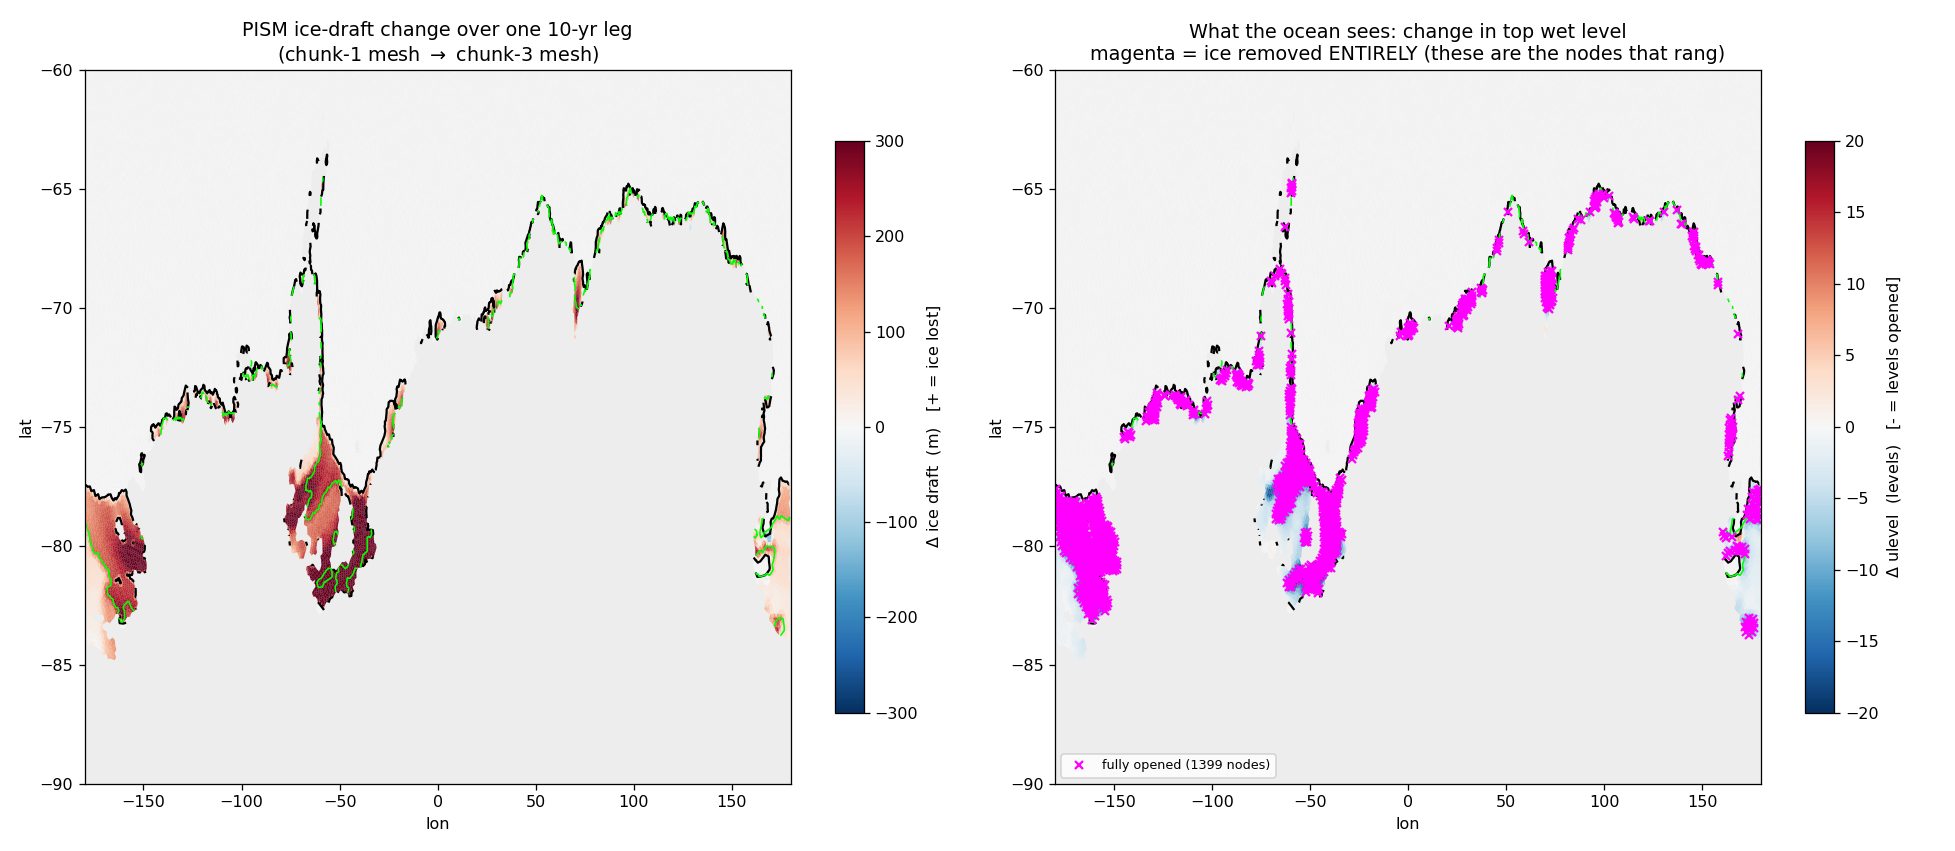
\includegraphics[width=\textwidth]{pism_change/pism_change_planview.png}
\end{center}

\begin{center}
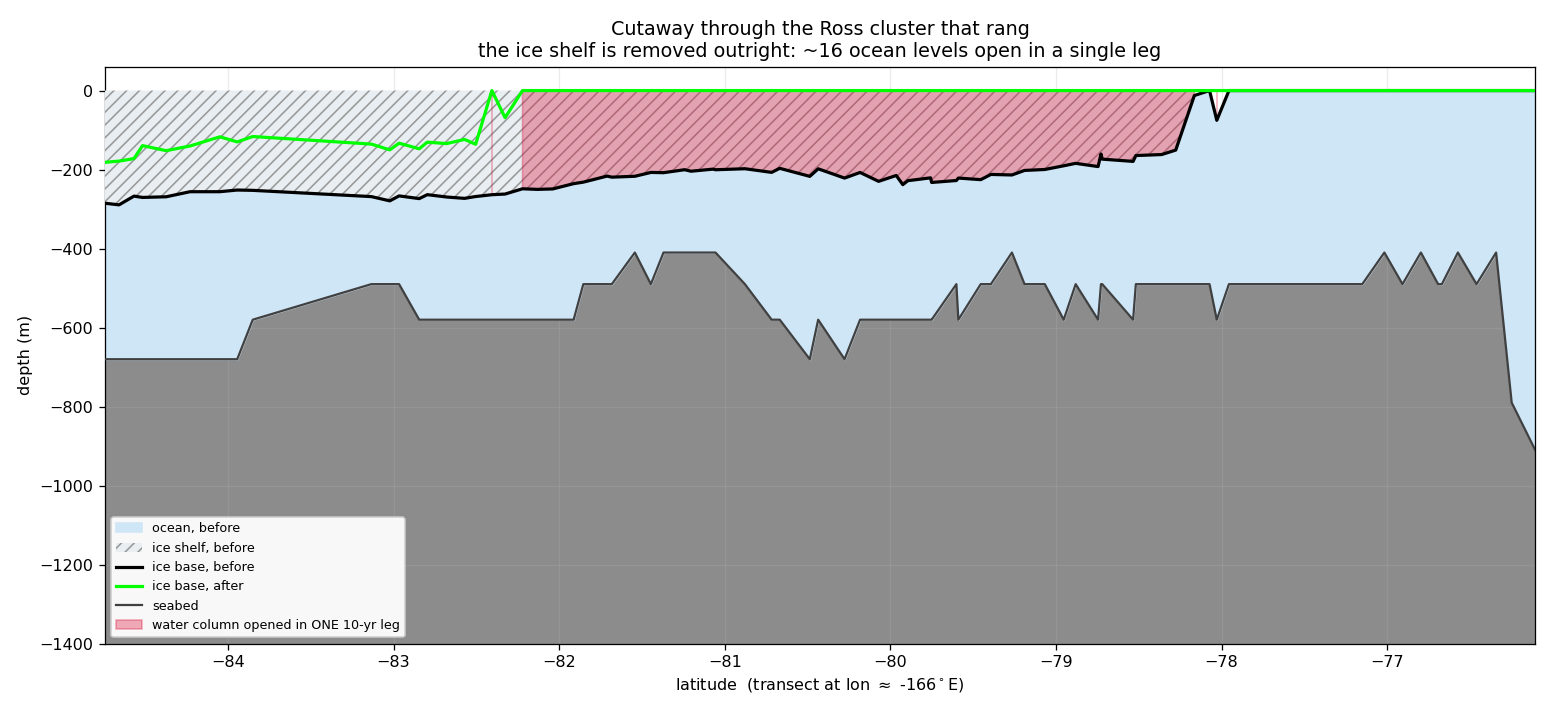
\includegraphics[width=0.92\textwidth]{pism_change/pism_change_section.png}
\end{center}

\noindent
The cutaway is the clearest statement of the problem: along this transect the ice base goes from
$-200\ldots-280$~m to \textbf{zero (open ocean)} across the whole span $-82.2^\circ$ to
$-78.2^\circ$~latitude. \textbf{The Ross ice-shelf front retreats $\approx$4$^\circ$ of latitude
($\approx$440~km) in ONE 10-yr leg.} The plan view shows this is not a Ross anomaly: the 1399
fully-opened nodes (magenta) ring the \emph{entire} Antarctic margin.

\begin{center}
\begin{tabular}{@{}lr@{}}
\toprule
changed nodes this leg & 3248 \quad(1.55\% of mesh) \\
$|\Delta \mathrm{ulev}| \ge 10$ & 1582 \\
\textbf{nodes with the ice removed ENTIRELY} & \textbf{1399} \\
\midrule
mean $|\Delta \mathrm{draft}|$ & \textbf{2.9\,m} \quad $\leftarrow$ \emph{meaningless} \\
max $|\Delta \mathrm{draft}|$ & \textbf{923\,m} \\
PISM floating cells & 24\,815 $\to$ 20\,093 \quad(\textbf{$-$24\% in 10~yr}) \\
\bottomrule
\end{tabular}
\end{center}

\noindent
\textbf{The mean is a lie.} It is diluted by the vast unchanged interior; the distribution is wildly
skewed. The earlier claim that a 10-yr PISM increment is a gentle $\approx$22\,m change --- which is
what motivated the entire ``sidestep the swap and the increments will be fine'' strategy --- was
\textbf{wrong}, and wrong in a way that mattered.

\medskip\noindent
PISM, started from the inherited spin-up state, is \textbf{not in equilibrium}: it is shedding ice
shelves catastrophically. No ocean model should be expected to swallow 440~km of ice-front retreat
in one coupling step.

\section{The encouraging half}

Of the \textbf{1399} nodes whose ice was removed outright, only \textbf{17 rang}. The ocean absorbed
$\sim$99\% of even \emph{this}, with the vertical-CFL transient peaking and then decaying. The remap
machinery --- which we have now shown to be bit-exact on unchanged nodes, inversion-free,
geometrically sound, and (after the fix below) free of manufactured values --- is performing far
better than a ``crashed at day 15'' headline suggests.

\section{A real remap bug fixed on the way}

The first attempt at this leg died at \textbf{mstep 1} with \code{found temperture becomes NaN or
<-5.0, >60}. The remapped restart contained $-45.02^\circ$C --- a value that exists \emph{nowhere} in
the source (wet range $[-2.32, 41.72]$, dry cells all $0.0$). The remap \emph{manufactured} it. The
column made the mechanism obvious:
\[
1.22,\ -0.99,\ -3.19,\ -5.39,\ -8.69,\ -13.09,\ -18.6,\ -25.2,\ -34.01,\ \mathbf{-45.02}
\]
Smooth and accelerating: an \textbf{unbounded linear extrapolation}. For columns that get
\emph{deeper} across a mesh change, the remap fitted a straight line through the last two old levels
and continued it downward with no clamp; over $\sim$9 new levels a thermocline slope compounds into
nonsense. Fixed by taking such water from the \emph{nearest old node actually wet at that depth} ---
the horizontal donor the rest of the remap already uses. Water below the old seabed should look like
the nearby ocean at that depth, not like a continuation of the local gradient.

\textbf{Never hit before} because every previous remap went mother\,$\to$\,submesh: the new mesh was
a strict \emph{subset}, so no column ever got deeper. Ice \emph{retreating} (208\,810 $\to$ 209\,172
nodes) exercises this path for the first time. (esm\_tools \code{eef4f6db}.)

\section{Where this leaves the strategy}

\begin{enumerate}
\item \textbf{Look at PISM first.} A run whose shelves collapse 24\%/decade is the anomaly. If PISM
      were equilibrated, the per-leg change would genuinely be small and the ocean side would very
      likely just work. \textbf{In particular: check the sub-shelf melt we are feeding PISM.} If our
      ocean hands PISM unrealistic melt, PISM's collapse is \emph{our} doing --- and that closes the
      loop.
\item \textbf{A per-leg $|\Delta\mathrm{ulev}|$ cap} is worth having as a robustness guard (defer the
      extreme tail across legs, so the ocean never sees 16 levels open at once). But it papers over
      a PISM problem rather than fixing one.
\item \textbf{The fully-opened column} is now a narrow, well-defined case (donor water + zero
      velocity + $\eta$ against still-cavity neighbours). Worth handling explicitly regardless.
\end{enumerate}

\section{Method note (continued)}

The ``mean $|\Delta\mathrm{draft}| = 22$\,m'' number was computed correctly and reported honestly ---
and was still deeply misleading, because a mean over a domain that is 98\% unchanged says nothing
about the tail that actually breaks the model. The distribution should have been plotted before it
was used to justify a strategy. Two figures did in ten minutes what a summary statistic obscured for
a day.

\end{document}
